% !TeX root = ./main.tex
\documentclass[main]{subfiles}
\begin{document}
\chapter{Топологические пространства}
\section{Топологические пространства}
\begin{example}
    В $\R^2$
    \begin{gather*}
        \rho_p ((x_1,y_1), (x_2, y_2)) = (|x_1 -x_2|^p + |y_1 - y_2|^p)^{1/p}\ \forall p \ge 1\\
        \rho_\infty = \max\{|x_1-x_2|; |y_1-y_2|\}\\
        \rho_{\text{срезающая}}(A,B) = \begin{cases}
            \rho_i (A,B) & \text{если } \rho_i (A, B) \le 1 \\
            1            & \text{если }\rho_i (A, B) > 1
        \end{cases}\\
        \rho' (A,B) = \frac{\rho(A,B)}{1 + \rho(A,B)},\ \rho'(A,B) < 1
    \end{gather*}
    У всех этих метрик одинаковые открытые множества

    Вывод: метрические пространства не всегда удобны.
\end{example}

\begin{definition}
    Пусть $X$ -- множество, а $\Omega$ -- система подмножеств $X$.
    ($\Omega \subset 2^X$ -- множество всех подмножеств $X$)
    Пара $(X,\Omega)$ называется топологическим пространством, если
    \begin{enumerate}
        \item $\forall \{U_i\}_{i \in I} \subset \Omega \implies \bigcup_{i \in I} U_i \in \Omega$
        \item $U_1, U_2 \in \Omega$, тогда $U_1 \cap U_2 \in \Omega$
        \item $\varnothing, X \in \Omega$
    \end{enumerate}
\end{definition}

\begin{definition}
    $\Omega$ называется топологией на $X$.
    Любое $U \in \Omega$ называется открытым подмножеством $X$.
\end{definition}

\begin{definition}
    $(X, \Omega)$ -- топологическое пространство. $F \subset X$. $F$ назовем замкнутым,
    если $X \setminus F$ -- открыто, т.е. $X \setminus F \in \Omega$.
\end{definition}

\begin{theorem}[Свойства замкнутых подмножеств]
    \

    \begin{enumerate}
        \item $\forall \{F_i\}_{i \in I}$ - замкнутые, то $\bigcap_{i\in I} F_i$ замкнутые
        \item $F_1, F_2$ -- замкнутые, то $F_1 \cup F_2$ замкнуты
        \item $\varnothing, X$ -- замкнуты
    \end{enumerate}
\end{theorem}
\begin{proof}
    Переход к дополнениям множеств и свойства объединения, пересечения и разности множеств.
\end{proof}

Таким образом топологическое пространство можно задавать при помощи замкнутых множеств.

\begin{example}
    Метрическая топология:  $(X, \rho)$ -- метрическое пространство, $\Omega$ -- множество всех открытых подмножеств.
    $U$ называет открытым, если $\forall x_0 \in U\ \exists \epsilon > 0: B(x_0, \epsilon) \coloneqq \{x \in X : \rho(x, x_0) < \epsilon\} \subset U$.
\end{example}

\begin{example}
    Дискретная топология: $X$ -- множество, $\Omega= 2^X$ (любое подмножество открыто).
\end{example}

\begin{example}
    Антидискретная топология: $X$ -- множество, $\Omega = \{ \varnothing, X\}$.
\end{example}

\begin{remark}
    2 пример -- частный случай 1-ого.
    \begin{gather*}
        \rho(x,y)  = \begin{cases}
            0 & x = y    \\
            1 & x \neq y
        \end{cases}\\
        B(x_0, 1/2) = \{x_0\} \text{ -- открыто}
    \end{gather*}
    А если любая точка открыта, значит любое подмножество открыто
\end{remark}

\begin{definition}
    Топология называется метризуемоей, если существует метрика $\rho$, порождающая
    данную топологию.
\end{definition}

Антидискретная топология не метризуема.
\begin{gather*}
    a, b \in X. \ r \coloneqq \rho(a,b). \ b \not\in B(a, r/2), a \in  B(a, r/2)\\
    B(a, r/2) \text{ -- открыто}
\end{gather*}

Вопрос: $(X, \Omega)$ -- топологическое пространство. Выяснить является ли
оно метризуемым.

\begin{example}
    Топология конечных дополнений (Зариского). $X$ -- бесконечное множество.
    $F$ называется замкнутым, если $F$ конечное или $F=X$.
    $\Omega \coloneqq \{X \setminus F: F \text{ конечно или $F=X$}\}$
\end{example}

\begin{theorem}[Гильберта о базисе] \label{space:gilbert}
    Любой идеал $I \subset F[x_1, x_2, ..., x_n]$ порождается конечным набором многочленов.
\end{theorem}

\begin{example}
    Развитие предыдущего примера. $F$ -- поле (в алгебраическом смысле).
    $F^n = F \times F \times ... \times F$ -- координатное пространство.
    $f_1, f_2, ..., f_k$ -- некоторые многочлены от $n$ переменных c коэффициентами в поле $F$.
    Тогда множество совместных корней этих многочленов назовем замкнутым множеством:
    \[G = \{(x_1, x_2,..., x_n): \forall i = 1...k \  f_i (x_1,..., x_n) = 0\}\]
    Это семейство замкнутых множеств порождает топологию.
    \[I = \{f_1 g_1 + f_2 g_2 + ... + f_k g_k : g_i \text{ -- любые многочлены от $n$ переменных}\}\]
    идеал, порожденный $f_1,...,f_n$

    По теореме \ref{space:gilbert} возникает соответствие $G \leftrightarrow I$.
    Это биекция, только если $F$ алгебраически замкнуто (по теореме Гильберта о нулях).

    Зачем это надо?
    \begin{gather*}
        x^n + y^n - z^n = f(x,y,z)\\
        n > 2, F = \Q
    \end{gather*}
    Существуют ли корни этого многочлена?
    А это великая теорема Ферма.
    $x^n + y^n - z^n = 0$
    (Решения в $\Z$ существуют, н.р. $x=y=z=0$)
\end{example}

\begin{example}
    Стрелка. $X = \R$ (или $\R_+$).
    \[\Omega = \{(a, +\infty): a \in X\} \cup \{\varnothing\} \cup \{X\}\]
    Это топология.
\end{example}

\begin{example}
    $D$ -- множество бесконечно дифференцируемых функций с компактным носителем, т.е.
    $f(x) = 0$ если $|x|>M$. ($\forall f \in D\ \exists M>0$: если $|x|>M$, то $f(x)=0$).
    \begin{center}
        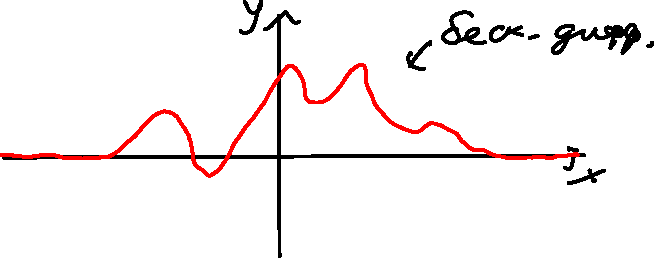
\includegraphics[width=0.7\linewidth]{inf_diff.pdf}
    \end{center}
    \[f_n(x) \rightrightarrows f(x) \text{ если } \forall \epsilon>0\ \exists N \in \N:
        \forall n \ge N\ |f_n(x) - f(x)| < \epsilon\ \forall x\]
    Пусть $f_n(x)$ -- последовательность функций в $D$. $f_n(x) \xrightarrow{D} f(x)$, если
    \begin{enumerate}
        \item $\exists M: \forall |x|>M\ \forall n\ f_n(x) = 0$
        \item $f_n(x) \rightrightarrows f(x); f_n'(x) \rightrightarrows f'(x)$ и т.д.
    \end{enumerate}
    $F \subset D$ называется замкнутым, если из $\{f_n(x)\}_{n\in \N} \subset F$
    и $f_n(x) \to f(x)$, следует $f(x) \in F$. Это порождает топологию на $D$.
\end{example}

\section{Расположение точки относительно множества}

\begin{definition}
    $(X, \Omega)$  -- топологическое пространство.  $x_0 \in X$.
    Окрестностью точки $x_0$ называется любое открытое подмножество $U_{x_0}: x_0 \in U_{x_0}$.
\end{definition}

\begin{definition}
    $A \subset X$ -- подмножество. $x_0 \in X$.

    $x_0$ -- внутренняя точка для $A$, если $\exists$ окрестность $U_{x_0} \subset A$

    $x_0$ -- внешняя точка $A$, если есть окрестность $U_{x_0} \cap A = \varnothing$ (т.е. $U_{x_0} \subset X \setminus A$)

    $x_0$ называется граничной, если $\forall U_{x_0}$ неверно $U_{x_0} \subset A$ и неверно $U_{x_0} \subset X \setminus A$.
    \begin{center}
        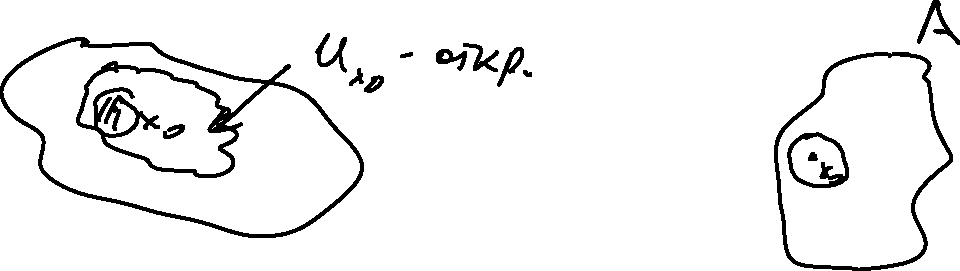
\includegraphics[width=0.7\linewidth]{top_neighborhood.pdf}
    \end{center}
\end{definition}

\begin{definition}
    $\Int A = \{x_0 \in X: x_0 \text{ --  внутренняя для } A\}$

    $\Ex A = \{x_0 \in X: x_0 \text{ --  внешняя для } A\}$

    $\partial A = \{x_0 \in X: x_0 \text{ --  граничная для } A\}$

    $\Cl A = \Int A \cup \partial A$
\end{definition}

\begin{theorem}
    \

    \begin{enumerate}
        \item $\displaystyle \Int A = \bigcup_{\substack{U_i \in \Omega \\ U_i \subset A}} U_i$
        \item $\displaystyle \Ex A = \bigcup_{\substack{U_i \in \Omega\\ U_i \cap A = \varnothing}} U_i$
        \item $\displaystyle \Cl A = \bigcap_{\substack{Z_i \text{ -- замкнуто} \\ A \subset Z_i}} Z_i$
    \end{enumerate}
\end{theorem}

\begin{remark}
    Часто именно это дается в качестве определения $\Int A$, $\Ex A$, $\Cl A$, $\partial A = \Cl A \setminus \Int A$
\end{remark}

\begin{proof}
    Докажем 1: заметим, что $\displaystyle \bigcup_{\substack{U_i \in \Omega \\ U_i \subset A}} U_i \supset \Int A$.

    Потому что $\Int A$ -- множество внутренних точек, а каждая такая точка входит вместе
    с окрестностью. Значит все окрестности включаются в левую часть.

    Почему $\displaystyle \bigcup_{\substack{U_i \in \Omega \\ U_i \subset A}} U_i \subset \Int A$?

    Возьмем $x_0$ из левой части, тогда $x_0 \in U_i \subset A$, значит $U_i$ нужная окрестность, чтобы считать $x_0$ внутренней.

    Докажем 2: аналогично 1.

    Докажем 3: следует из 1 потому что $U_i \coloneqq X \setminus F_i$.
    \begin{multline*}
        \bigcap_{\substack{F_i \text{ -- замкнуто} \\ A \subset  F_i}} F_i =
        \bigcap_{\substack{U_i \text{ -- открыто}\\ U_i \cap A = \varnothing \\ U_i \subset X \setminus A}} (X \setminus U_i) =
        X \setminus \bigcup_{\substack{U_i \in \Omega\\ U_i \subset X \setminus A}} U_i = \\
        X \setminus \Ex A = \Cl A
    \end{multline*}
\end{proof}

\section{Базы и предбазы}
\begin{definition}
    $(X, \Omega)$ -- топологическое пространство. $\mathfrak{B} \subset 2^X$ (Точнее $\mathfrak{B}\subset \Omega$).
    $\mathfrak{B}$ называется базой топологии $\Omega$, если
    \[\forall U \in \Omega \quad U = \bigcup_{i \in I}B_i \ (\exists I\ \exists B_i): B_i \in \mathfrak{B}.\]
\end{definition}

\begin{definition}
    $\mathfrak{B}$ называется базой некоторой топологии, если существует
    $\Omega : \mathfrak{B}$ база топологии.
\end{definition}
\begin{remark}
    Такая $\Omega$ единственна:
    \[\Omega = \left\{\bigcup_{i \in I} B_i: B_i \in \mathfrak{B}\right\}.\]
\end{remark}

\begin{example}
    В $\R^n$ $\mathfrak{B} \coloneqq \{ B(x, \epsilon): x \in R^n; \epsilon>0\}$.
    $\R^n$ можно заменить на любое метрическое пространство.
\end{example}
\begin{example}
    $X = \N$. $\mathfrak{B}$ -- множество арифметических прогрессий, тогда $\mathfrak{B}$ база
    некоторой топологии. (обоснование позже)
\end{example}
\begin{example}
    $(X, \Omega)$ -- дискретное пространство. $\mathfrak{B}$ все одноточечные множества.
    $\mathfrak{B}$ -- база $\Omega$.
\end{example}
\begin{example}
    $C(\R^n)$ -- множество непрерывных функций из $\R^n \to \R$. (Это обобщается)

    $K_1, ..., K_n$ -- замкнутые и ограниченные подмножества $\R^n$.
    $U_1, ..., U_n$ -- открытые множества в $\R$.
    \[V_{K_1, ..., K_n}^{U_1, ..., U_n} \coloneqq \{f: \R^n \to \R\text{ -- непрерывно} : f(K_i) \subset U_i, i = 1,..., n\}\]
    Множество таких $V_{K_1, ..., K_n}^{U_1, ..., U_n}$ -- база некоторой топологии.
    Она называется компактно-открытая топология.
\end{example}

\begin{theorem}
    $(X, \Omega)$ -- топологическое пространство, $\mathfrak{B} \subset \Omega$, то $\mathfrak{B}$ -- база $\Omega$
    $\Leftrightarrow \forall U \in \Omega\ \forall x_0 \in U\ \exists B \in \mathfrak{B}: x_0\in B\subset U$.
\end{theorem}
\begin{proof}
    $U = \bigcup_{x_0 \in U} B_{x_0}$
\end{proof}

\begin{theorem}
    $X$ -- множество, $\mathfrak{B} \subset 2^X$. $\mathfrak{B}$ является базой некоторой топологии
    \[\Leftrightarrow \forall B_1, B_2 \in \mathfrak{B}\ \forall x_0 \in B_1 \cap B_2\ \exists B_3 \in \mathfrak{B}: x_0 \in B_3 \subset B_1 \cap B_2\]
    и $\bigcup_{B \in \mathfrak{B}} B = X$.
\end{theorem}
\begin{remark}
    Частный случай: Если $B_1 \cap B_2 \in \mathfrak{B}$, то $\mathfrak{B}$ -- база топологии.
\end{remark}
\begin{proof}
    Прямое доказательство: по предыдущей теореме. ($U \coloneqq B_1 \cap B_2$)

    Обратное доказательство: $\Omega \coloneqq \left\{\bigcup_{i \in I} B_i: B_i \in \mathfrak{B}\right\}$.
    $\Omega$ -- топология?
    \begin{enumerate}
        \item $U_i = \bigcup_{j \in J_i} B_{ij}$, ($B_{ij} \in \mathfrak{B}$), тогда
              \[\bigcup_{i \in I} U_i = \bigcup_{i \in I} \bigcup_{j \in J} B_{ij} \in \Omega\]
        \item $U_1 = \bigcup_{i \in I} B_i$, $U_2 = \bigcup_{j \in J} C_j$, $B_i, C_j \in \mathfrak{B}$, $B_i \cap C_j = \bigcup_{x_0 \in B_i \cap C_j} B_3 (x_0)$

              Почему $U_1 \cap U_2 \in \Omega$?
              \begin{multline*}
                  U_1 \cap U_2 = \left(\bigcup_{i \in I} B_i\right) \cap \left(\bigcup_{j \in J} C_j\right) = \bigcup_{(i,j) \in I \times J} (B_i \cap C_j) = \\
                  \bigcup_{(i,j)} \bigcup_{x_0 \in B_i \cap C_j} B_3 (x_0; B_i \cap C_j) \in \Omega
              \end{multline*}
              и каждое $B_3 (x_0; B_i \cap C_j) \in \mathfrak{B}$
        \item $\varnothing = \bigcup_{i \in \varnothing} B_i$, $X = \bigcup_{B \in \mathfrak{B}} B$
    \end{enumerate}
\end{proof}

\begin{definition}
    $(X, \Omega)$ -- топологическое пространство. $\mathfrak{A}$ называется предбазой $\Omega$, если
    $\mathfrak{B} \coloneqq \{\bigcap_{i = 1}^n A_i : A_i \in \mathfrak{A}\}$ -- база $\Omega$.

    То есть предбаза -- любой набор подмножеств, объединение которых $X$.
\end{definition}

\begin{definition}
    $(X, \Omega)$ -- топологическое пространство.
    $\forall x_0 \in X$ задано $\mathfrak{B}_{x_0}$ -- множество некоторых окрестностей $x_0$.
    $\mathfrak{B}_{x_0} \in \Omega$.
    Говорим, что $\{\mathfrak{B}_{x_0}\}_{x_0 \in X}$ является базой окрестностей точек $\Omega$,
    если $\forall U \in \Omega\ \forall x_0 \in X: x_0 \in U\ \exists B(x_0, U) \in \mathfrak{B}_{x_0}:
        x_0 \in B(x_0, U) \subset U$.
\end{definition}
\begin{remark}
    $\bigcup_{x_0 \in X} \mathfrak{B}_{x_0}$ -- база $\Omega$.
    \[U = \bigcup_{x_0 \in U} B(x_0, U)\]
\end{remark}
\begin{example}
    $(M, \rho)$ -- метрическое пространство, тогда $\mathfrak{B}_{x_0} = \{B(x_0, \epsilon) : \epsilon > 0\}$.
\end{example}

\begin{theorem}
    $X$ -- множество. $\forall x_0 \in X\ \exists \mathfrak{B}_{x_0} \subset 2^X$: ($\mathfrak{B}_{x_0} \neq \varnothing$)
    \begin{enumerate}
        \item $\forall B \in \mathfrak{B}_{x_0}\ x_0 \in B$
        \item $\forall B_1, B_2 \in \mathfrak{B}_{x_0} \implies \exists B_3 \in \mathfrak{B}_{x_0}: B_3 \in B_1 \cap B_2$
        \item $\forall B_1 \in \mathfrak{B}_{x_0}, \forall x_1 \in B_1\ \exists B_2 \in \mathfrak{B}_{x_1}: x_1 \in B_2 \subset B_1$
    \end{enumerate}
    Если все это выполнено, то $\bigcup_{x_0 \in X} \mathfrak{B}_{x_0}$ -- база некоторой топологии.
\end{theorem}
\begin{proof}
    Смотри предыдущую теорему.
\end{proof}
\end{document}